
\section{Moving angle system}\label{sec:servo_model}


The use of a tracking antenna system requires a device to change the orientation of the antennas. The moving angle system is performing this task and is composed of a DC servomotor for the rotational movement of the antennas, a gear to have a precise change of the angles, and a sensor to keep track of the actual angle and compare it to the reference.

The DC servomotor, presented in the section \ref{sec:servo_motor}, can be divided in two different groups: the DC motor and the servomechanism.

DC motor is an actuator which converts electrical energy to mechanical rotation. In the figure \ref{dcmotor_circuit} it is possible to see the model of this motor. DC motors are a type of motors which were built to receive a voltage as an input and, after converting this voltage, to apply a specific velocity on its shaft. In other words, DC motors are able to control the velocity of the shaft.

\begin{figure}[H]
\centering
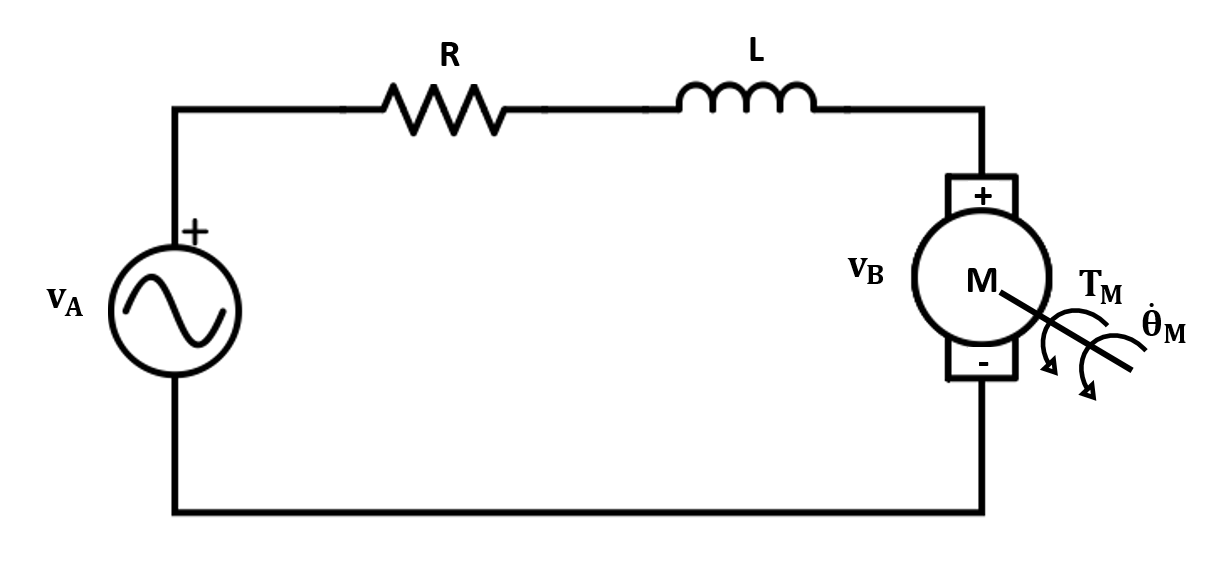
\includegraphics[scale=0.5]{figures/dcmotor_circuit.png}
\caption{Circuit of the DC motor}
\label{dcmotor_circuit}
\end{figure}

The circuit of the previous figure is described by the equations \ref{DC_motor_equation1}, \ref{DC_motor_equation2} and \ref{DC_motor_equation3}. It is possible to observe that between the source unit and the motor there are two elements (resistance and inductance). These elements are important due to the fact that they are the responsible for the stability of the system, avoiding a motor overload. Hence, the relation between the current and the difference between the voltage of the source and the one of the motor is made through an admitance.

\begin{equation}\label{DC_motor_equation1}
v_{a}= v_{b}+i_{a} R_{a}+L_{a}\frac{\mathrm{d} i_{a}}{\mathrm{d} t}
\end{equation}

\begin{equation}\label{DC_motor_equation2}
V_{a}(s)= V_{b}(s)+I_{a}(s) R_{a}+sL_{a}I_{a}(s)
\end{equation}

\begin{equation}\label{DC_motor_equation3}
I_{a}(s)= \frac{V_{a}(s)-V_{b}(s)}{R_{a}+sL_{a}} , I_{a}(s)= G_{I}(V_{a}(s)-V_{b}(s))
\end{equation}

The model of the figure \ref{model1} is the representation of the equation \ref{DC_motor_equation3}.

\begin{figure}[H]
\centering
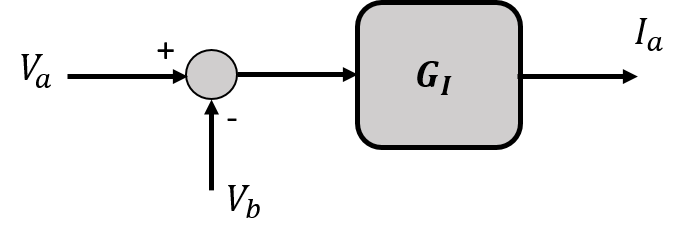
\includegraphics[scale=0.6]{figures/model1.png}
\caption{Relation between the input and the feedback voltage and the current of the circuit}
\label{model1}
\end{figure}

Furthermore, the sum of torques applied on the motor depends on the load attached to the motor shaft. The inertial and damping behaviours of the load can be represented as a inertia coefficient, $J_{e}$, and a viscous damping coefficient, $D_{e}$. This total tendency of a force to rotate an object about an axis is represented by $T_{m}$ which is described through the equation \ref{torque_time}. 

\begin{equation}\label{torque_time}
T_{m}(t)= J_{e}\frac{\mathrm{d} \dot{\theta}_{m}(t)}{\mathrm{d} t}+D_{e}\dot{\theta}_{m}(t)
\end{equation}

However, the servomotor is a type of motor which is able to control the position of the shaft. Using a potentiometer it is possible to send an electrical signal with the information about the angle. Thus, using the relation between the velocity and the position described in the equation \ref{theta_relation}, it is possible to write the equation \ref{torque_frequency_theta}.

\begin{equation}\label{theta_relation}
\dot{\theta}_{m}(s)= s\theta_{m}(s)
\end{equation}

\begin{equation}\label{torque_frequency_theta}
T_{m}(s)= (s^{2}J_{e} + sD_{e})\theta_{m}(s)
\end{equation}

The torque is also proportional to the current that passes through the circuit. The constant of proportionality is called torque constant and the relation between the torque and the current is presented in the equations \ref{torque_curr1} and \ref{torque_curr2}.

\begin{equation}\label{torque_curr1}
T_{m}(t)= K_{t} i_{a}(t)
\end{equation}

\begin{equation}\label{torque_curr2}
T_{m}(s)= K_{t} I_{a}(s)
\end{equation}

Based on the previous equations and on the model in the figure \ref{model1} it is possible to build the model in the figure \ref{model2}.

\begin{figure}[H]
\centering
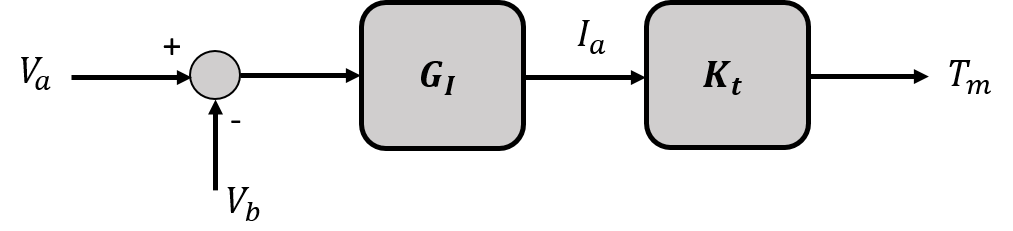
\includegraphics[scale=0.6]{figures/model2.png}
\caption{Relation between the voltage and the applied torque}
\label{model2}
\end{figure}

The applied torque $T_{m}(s)$ described in the previous equations can be also related to the angle position $\theta_{m}(s)$ through the equations \ref{torque_frequency} and \ref{torque_frequency_G}.

\begin{equation}\label{torque_frequency}
T_{m}(s) I_{a}(s)= (s^{2}J_{e} + sD_{e})\theta_{m}(s)
\end{equation}

\begin{equation}\label{torque_frequency_G}
\theta_{m}(s)= G_{\theta}(s)\times T_{m}(s) , G_{\theta}(s)=\frac{1}{s^{2}J_{e} + sD_{e}}
\end{equation}

\begin{figure}[H]
\centering
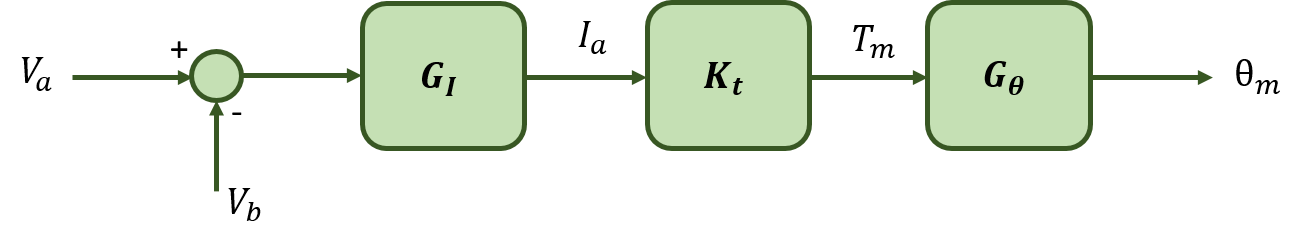
\includegraphics[scale=0.6]{figures/model3.png}
\caption{Relation between the voltage and the angle of the shaft}
\label{model3}
\end{figure}

Finally, it is also possible to calculate the relation between the output theta and voltage. Thus, the comparison between the output and the input voltage allows the formation of a closed loop using a feedback (figure \ref{model4}).

\begin{equation}\label{feedback1}
v_{b}(t)= K_{b}\frac{\mathrm{d} \theta_{m}(t)}{\mathrm{d} t}
\end{equation}

\begin{equation}\label{feedback2}
V_{b}(s)= sK_{b}\theta_{m}(s)
\end{equation}

\begin{figure}[H]
\centering
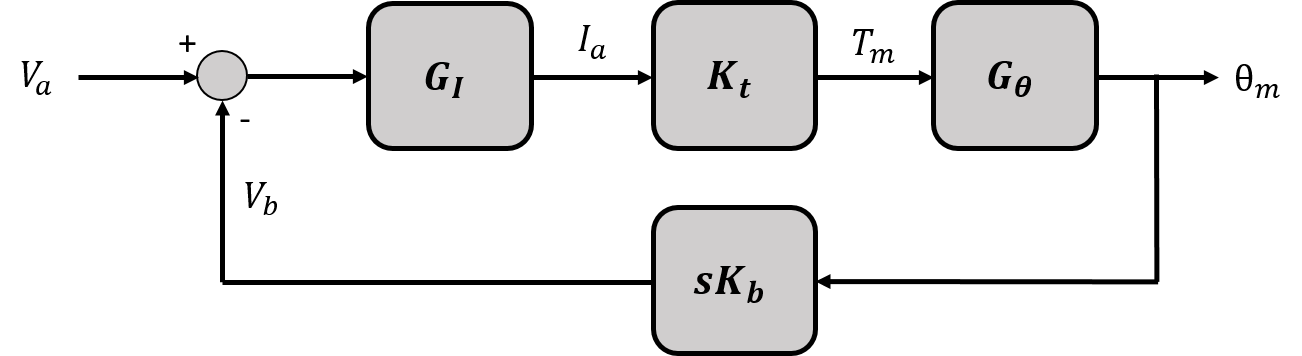
\includegraphics[scale=0.6]{figures/model4.png}
\caption{Model of a servomotor}
\label{model4}
\end{figure}

A gear was added to the servomotor to reduce its speed and obtain a better precision for the output angle. Time to reach the desired angle and required precision were taken into account to choose a gear ratio.
For instance, a gear ratio of 0.001 means that 1000 rotations of the motor will result in a single rotation at the end of the system.

\begin{figure}[H]
\centering
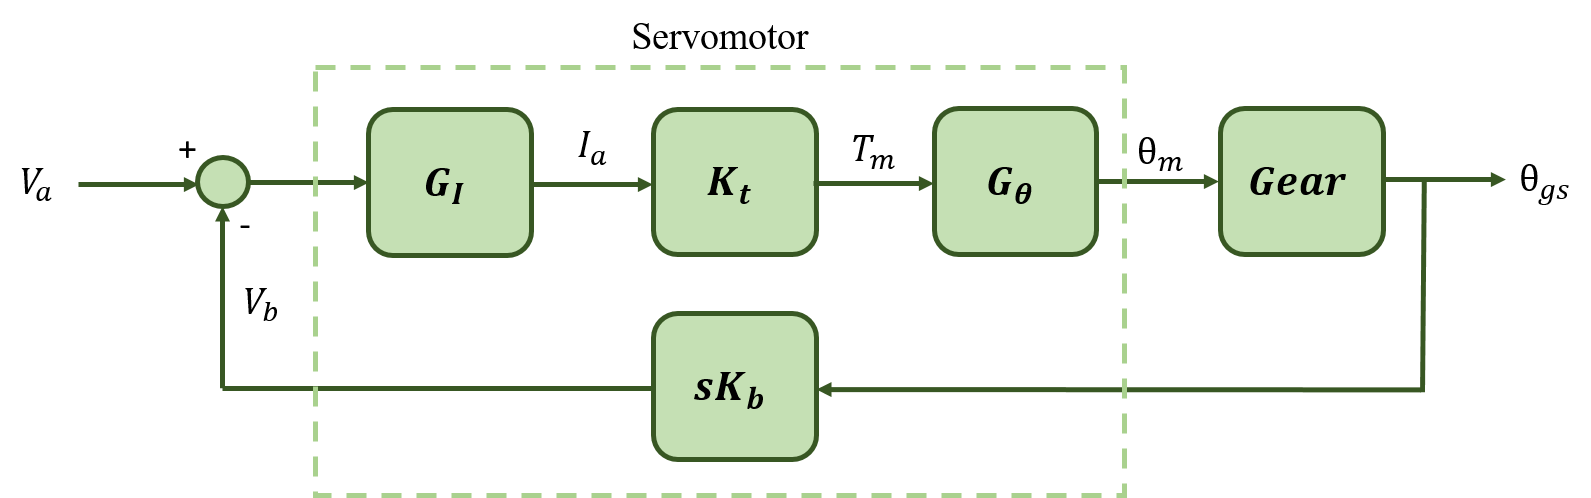
\includegraphics[scale=0.6]{figures/servo+gear.png}
\caption{Servomotor with a gear}
\label{model4}
\end{figure}

In order to control the antennas, the input of the system is the desired angle. However, the servomotor requires an electrical signal input (voltage) that represents the rotations needed. This voltage is the output of a controller whose input is a comparison between the reference angle and the actual one (error angle). The current angle of the system is given by a sensor.
Assuming that the sensor is not ideal, the disturbances caused by it can be simulated by adding a white noise to the feedback of the plant.

\begin{figure}[H]
\centering
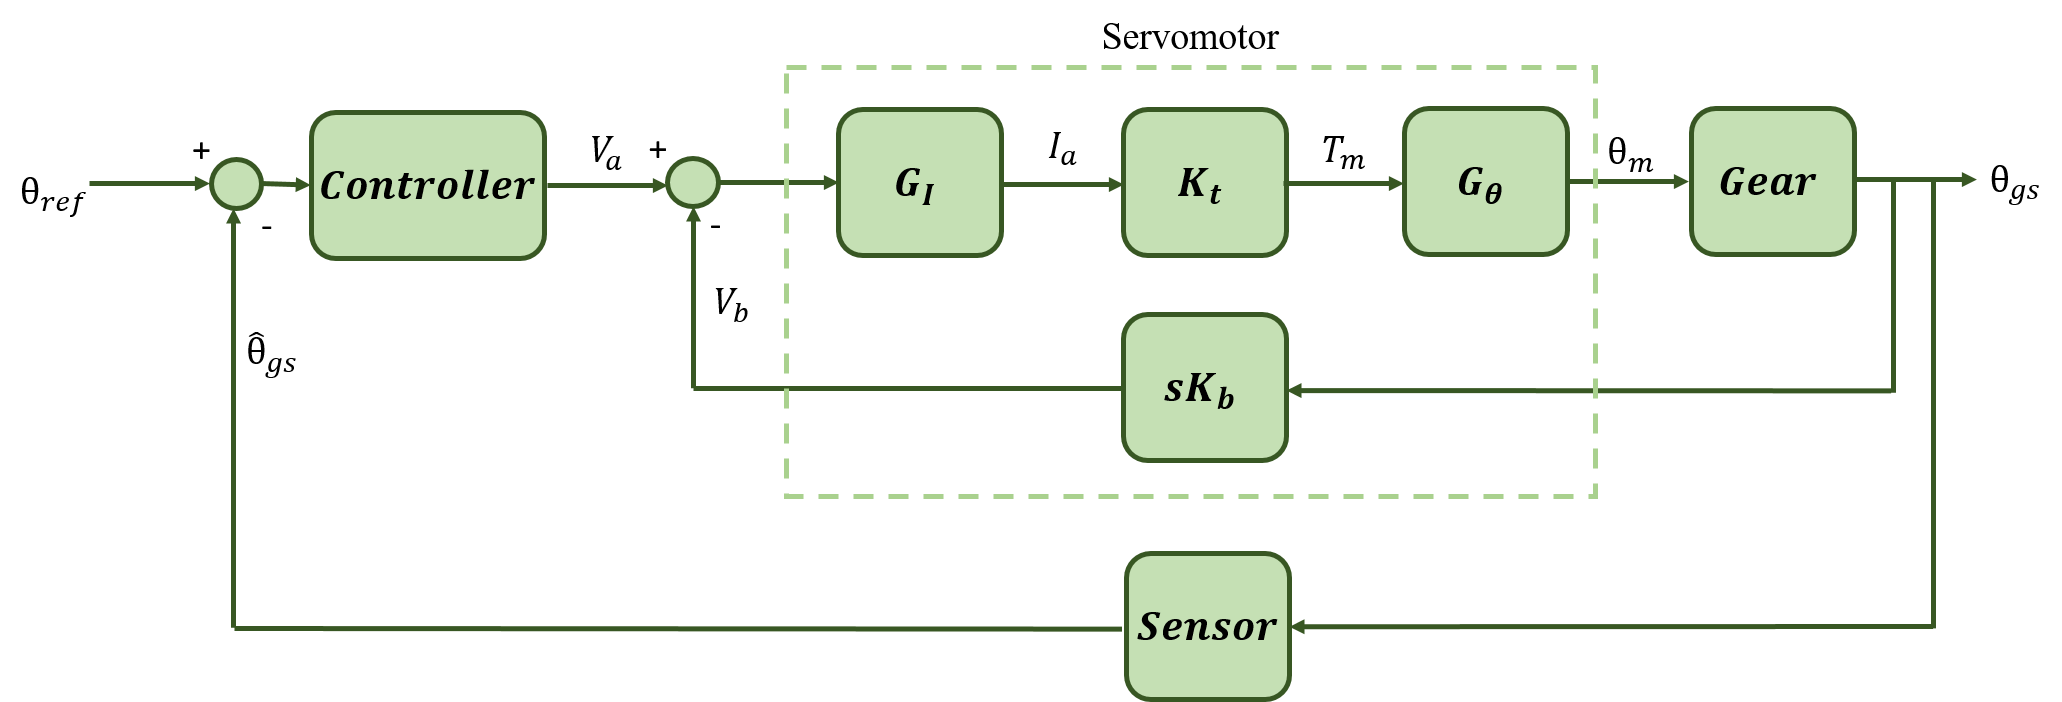
\includegraphics[scale=0.5]{figures/servo+gear+noise.png}
\caption{Limitation of the voltage into the servomotor and its gear}
\label{model4}
\end{figure}

High voltage value can be the consequence of the controller trying to reach the desired value in the fastest way. With a view to procure a range of voltage that the motor can handle and prevent any damage, a saturation box was included.

\begin{figure}[H]
\centering
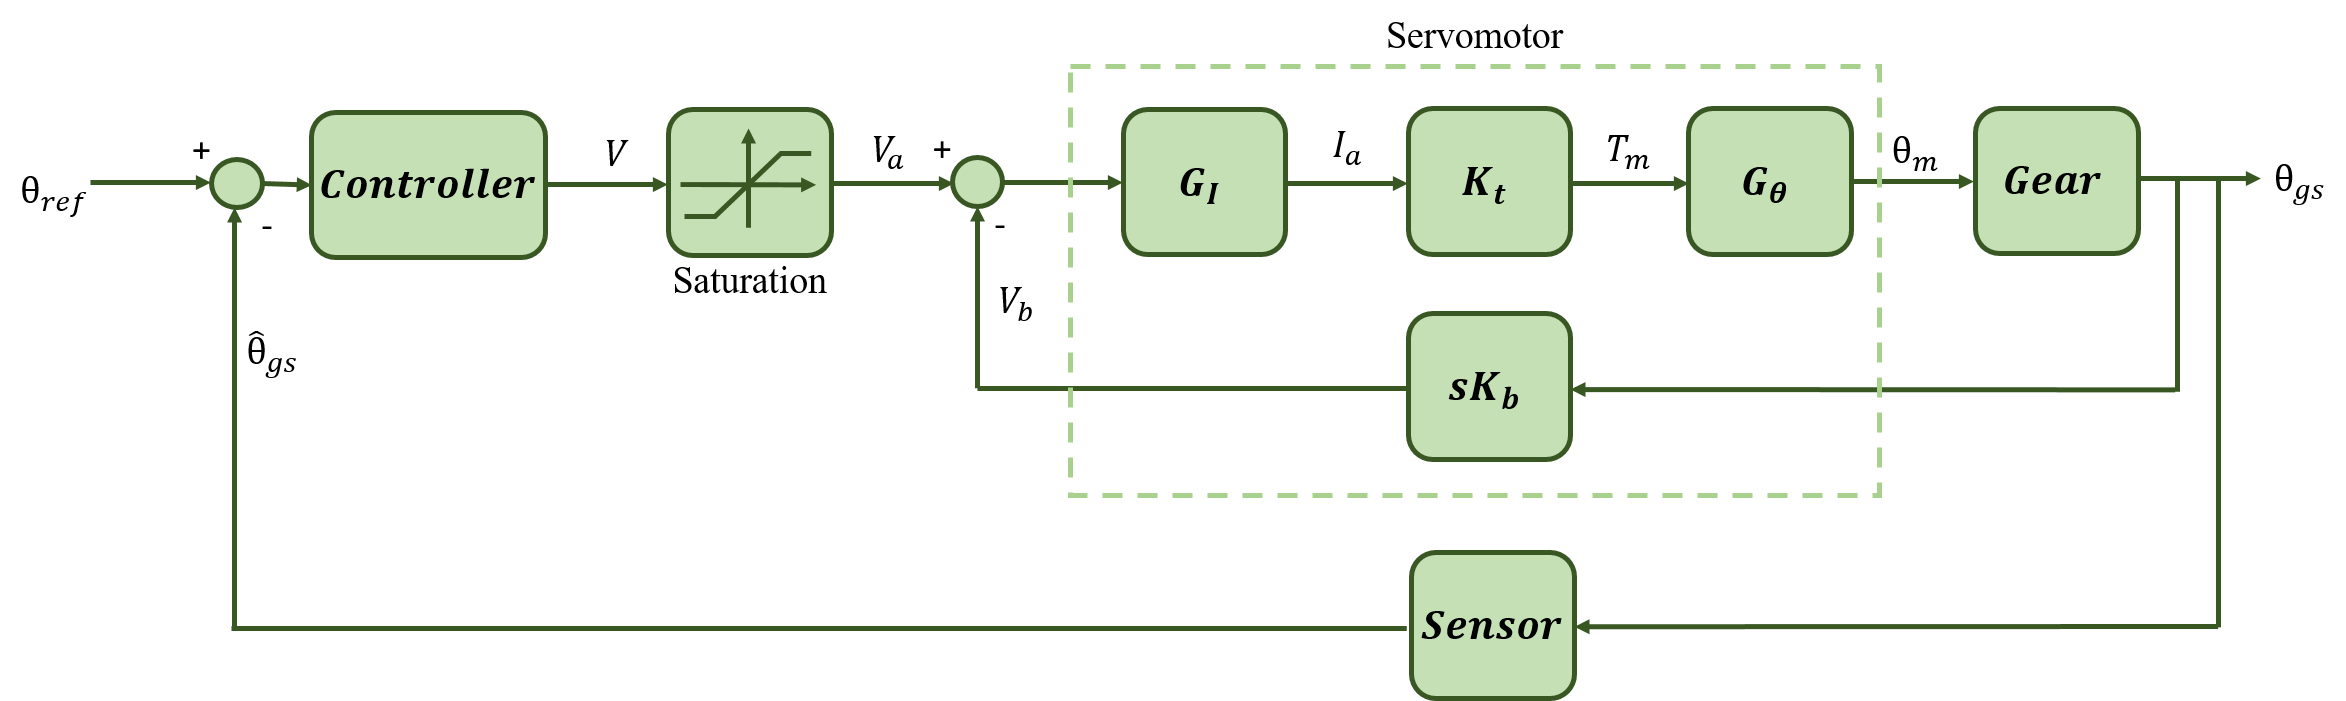
\includegraphics[scale=0.4]{figures/complete_model.png}
\caption{Model of the Moving Angle System}
\label{model4}
\end{figure}

Figure \ref{model4} shows the integral plant of the Moving Angle System. This model was used in \emph{Simulink} to test the behavior of the system and was later included in the 3D system simulation, described in section \ref{sec:3d_sim}. The reference angles and the adopted controller are explained in the followings sections.